\chapter{Búsqueda exhaustiva}

\key{Búsqueda exhaustiva}
es un método general que se puede utilizar
para resolver casi cualquier problema algorítmico.
La idea es generar todas las posibles
soluciones al problema mediante fuerza bruta,
y luego seleccionar la mejor solución o contar el
número de soluciones, dependiendo del problema.

La búsqueda exhaustiva es una buena técnica
si hay suficiente tiempo para revisar todas las soluciones,
ya que la búsqueda suele ser fácil de implementar
y siempre proporciona la respuesta correcta.
Si la búsqueda exhaustiva es demasiado lenta,
pueden ser necesarias otras técnicas, como algoritmos voraces o
programación dinámica.

\section{Generando subconjuntos}

\index{subconjunto}

Primero consideramos el problema de generar
todos los subconjuntos de un conjunto de $n$ elementos.
Por ejemplo, los subconjuntos de $\{0,1,2\}$ son
$\emptyset$, $\{0\}$, $\{1\}$, $\{2\}$, $\{0,1\}$,
$\{0,2\}$, $\{1,2\}$ y $\{0,1,2\}$.
Hay dos métodos comunes para generar subconjuntos:
podemos realizar una búsqueda recursiva
o aprovechar la representación en bits de los enteros.

\subsubsection{Método 1}

Una forma elegante de recorrer todos los subconjuntos
de un conjunto es utilizar recursión.
La siguiente función \texttt{busqueda}
genera los subconjuntos del conjunto
$\{0,1,\ldots,n-1\}$.
La función mantiene un vector \texttt{subconjunto}
que contendrá los elementos de cada subconjunto.
La búsqueda comienza cuando se llama
a la función con el parámetro 0.

\begin{lstlisting}
void busqueda(int k) {
    if (k == n) {
        // procesar subconjunto
    } else {
        busqueda(k+1);
        subconjunto.push_back(k);
        busqueda(k+1);
        subconjunto.pop_back();
    }
}
\end{lstlisting}

Cuando se llama a la función \texttt{busqueda}
con el parámetro $k$,
decide si incluir o no el
elemento $k$ en el subconjunto,
y en ambos casos,
luego se llama a sí misma con el parámetro $k+1$.
Sin embargo, si $k=n$, la función se da cuenta de que
todos los elementos han sido procesados
y se ha generado un subconjunto.

El siguiente árbol ilustra las llamadas a funciones cuando $n=3$.
Siempre podemos elegir la rama izquierda
($k$ no está incluido en el subconjunto) o la rama derecha
($k$ está incluido en el subconjunto).

\begin{center}
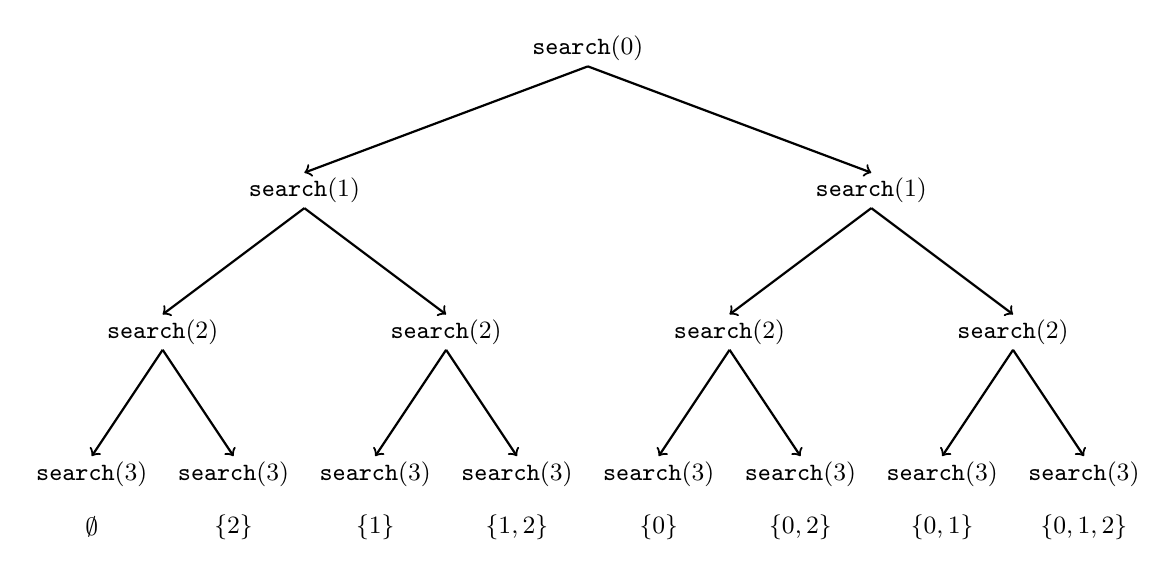
\begin{tikzpicture}[scale=.45]
  \begin{scope}
    \small
    \node at (0,0) {$\texttt{search}(0)$};

    \node at (-8,-4) {$\texttt{search}(1)$};
    \node at (8,-4) {$\texttt{search}(1)$};

    \path[draw,thick,->] (0,0-0.5) -- (-8,-4+0.5);
    \path[draw,thick,->] (0,0-0.5) -- (8,-4+0.5);

    \node at (-12,-8) {$\texttt{search}(2)$};
    \node at (-4,-8) {$\texttt{search}(2)$};
    \node at (4,-8) {$\texttt{search}(2)$};
    \node at (12,-8) {$\texttt{search}(2)$};

    \path[draw,thick,->] (-8,-4-0.5) -- (-12,-8+0.5);
    \path[draw,thick,->] (-8,-4-0.5) -- (-4,-8+0.5);
    \path[draw,thick,->] (8,-4-0.5) -- (4,-8+0.5);
    \path[draw,thick,->] (8,-4-0.5) -- (12,-8+0.5);

    \node at (-14,-12) {$\texttt{search}(3)$};
    \node at (-10,-12) {$\texttt{search}(3)$};
    \node at (-6,-12) {$\texttt{search}(3)$};
    \node at (-2,-12) {$\texttt{search}(3)$};
    \node at (2,-12) {$\texttt{search}(3)$};
    \node at (6,-12) {$\texttt{search}(3)$};
    \node at (10,-12) {$\texttt{search}(3)$};
    \node at (14,-12) {$\texttt{search}(3)$};

    \node at (-14,-13.5) {$\emptyset$};
    \node at (-10,-13.5) {$\{2\}$};
    \node at (-6,-13.5) {$\{1\}$};
    \node at (-2,-13.5) {$\{1,2\}$};
    \node at (2,-13.5) {$\{0\}$};
    \node at (6,-13.5) {$\{0,2\}$};
    \node at (10,-13.5) {$\{0,1\}$};
    \node at (14,-13.5) {$\{0,1,2\}$};


    \path[draw,thick,->] (-12,-8-0.5) -- (-14,-12+0.5);
    \path[draw,thick,->] (-12,-8-0.5) -- (-10,-12+0.5);
    \path[draw,thick,->] (-4,-8-0.5) -- (-6,-12+0.5);
    \path[draw,thick,->] (-4,-8-0.5) -- (-2,-12+0.5);
    \path[draw,thick,->] (4,-8-0.5) -- (2,-12+0.5);
    \path[draw,thick,->] (4,-8-0.5) -- (6,-12+0.5);
    \path[draw,thick,->] (12,-8-0.5) -- (10,-12+0.5);
    \path[draw,thick,->] (12,-8-0.5) -- (14,-12+0.5);
\end{scope}
\end{tikzpicture}
\end{center}

\subsubsection{Method 2}

Another way to generate subsets is based on
the bit representation of integers.
Each subset of a set of $n$ elements
can be represented as a sequence of $n$ bits,
which corresponds to an integer between $0 \ldots 2^n-1$.
The ones in the bit sequence indicate
which elements are included in the subset.

The usual convention is that
the last bit corresponds to element 0,
the second last bit corresponds to element 1,
and so on.
For example, the bit representation of 25
is 11001, which corresponds to the subset $\{0,3,4\}$.

The following code goes through the subsets
of a set of $n$ elements

\begin{lstlisting}
for (int b = 0; b < (1<<n); b++) {
    // process subset
}
\end{lstlisting}

The following code shows how we can find
the elements of a subset that corresponds to a bit sequence.
When processing each subset,
the code builds a vector that contains the
elements in the subset.

\begin{lstlisting}
for (int b = 0; b < (1<<n); b++) {
    vector<int> subset;
    for (int i = 0; i < n; i++) {
        if (b&(1<<i)) subset.push_back(i);
    }
}
\end{lstlisting}

\section{Generating permutations}

\index{permutation}

Next we consider the problem of generating
all permutations of a set of $n$ elements.
For example, the permutations of $\{0,1,2\}$ are
$(0,1,2)$, $(0,2,1)$, $(1,0,2)$, $(1,2,0)$,
$(2,0,1)$ and $(2,1,0)$.
Again, there are two approaches:
we can either use recursion or go through the
permutations iteratively.

\subsubsection{Method 1}

Like subsets, permutations can be generated
using recursion.
The following function \texttt{search} goes
through the permutations of the set $\{0,1,\ldots,n-1\}$.
The function builds a vector \texttt{permutation}
that contains the permutation,
and the search begins when the function is
called without parameters.

\begin{lstlisting}
void search() {
    if (permutation.size() == n) {
        // process permutation
    } else {
        for (int i = 0; i < n; i++) {
            if (chosen[i]) continue;
            chosen[i] = true;
            permutation.push_back(i);
            search();
            chosen[i] = false;
            permutation.pop_back();
        }
    }
}
\end{lstlisting}

Each function call adds a new element to
\texttt{permutation}.
The array \texttt{chosen} indicates which
elements are already included in the permutation.
If the size of \texttt{permutation} equals the size of the set,
a permutation has been generated.

\subsubsection{Method 2}

\index{next\_permutation@\texttt{next\_permutation}}

Another method for generating permutations
is to begin with the permutation
$\{0,1,\ldots,n-1\}$ and repeatedly
use a function that constructs the next permutation
in increasing order.
The C++ standard library contains the function
\texttt{next\_permutation} that can be used for this:

\begin{lstlisting}
vector<int> permutation;
for (int i = 0; i < n; i++) {
    permutation.push_back(i);
}
do {
    // process permutation
} while (next_permutation(permutation.begin(),permutation.end()));
\end{lstlisting}

\section{Backtracking}

\index{backtracking}

A \key{backtracking} algorithm
begins with an empty solution
and extends the solution step by step.
The search recursively
goes through all different ways how
a solution can be constructed.

\index{queen problem}

As an example, consider the problem of
calculating the number
of ways $n$ queens can be placed on
an $n \times n$ chessboard so that
no two queens attack each other.
For example, when $n=4$,
there are two possible solutions:

\begin{center}
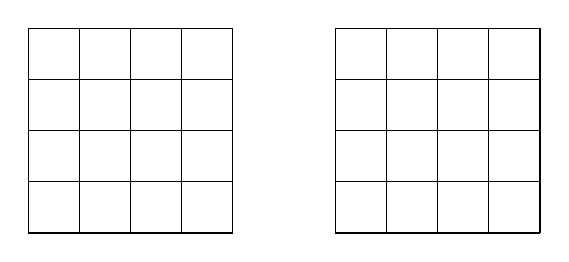
\begin{tikzpicture}[scale=.65]
  \begin{scope}
    \draw (0, 0) grid (4, 4);
    \node at (1.5,3.5) {\symqueen};
    \node at (3.5,2.5) {\symqueen};
    \node at (0.5,1.5) {\symqueen};
    \node at (2.5,0.5) {\symqueen};

    \draw (6, 0) grid (10, 4);
    \node at (6+2.5,3.5) {\symqueen};
    \node at (6+0.5,2.5) {\symqueen};
    \node at (6+3.5,1.5) {\symqueen};
    \node at (6+1.5,0.5) {\symqueen};

  \end{scope}
\end{tikzpicture}
\end{center}

The problem can be solved using backtracking
by placing queens to the board row by row.
More precisely, exactly one queen will
be placed on each row so that no queen attacks
any of the queens placed before.
A solution has been found when all
$n$ queens have been placed on the board.

For example, when $n=4$,
some partial solutions generated by
the backtracking algorithm are as follows:

\begin{center}
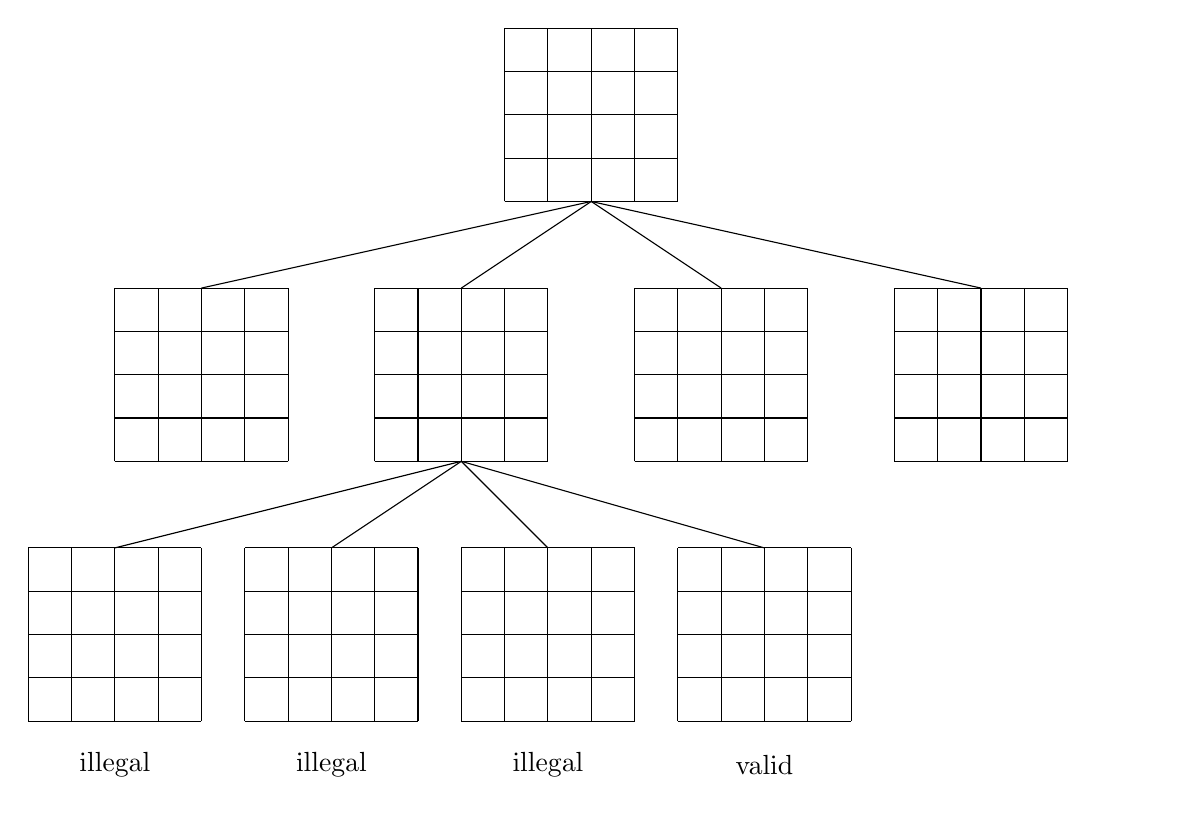
\begin{tikzpicture}[scale=.55]
  \begin{scope}
    \draw (0, 0) grid (4, 4);

    \draw (-9, -6) grid (-5, -2);
    \draw (-3, -6) grid (1, -2);
    \draw (3, -6) grid (7, -2);
    \draw (9, -6) grid (13, -2);

    \node at (-9+0.5,-3+0.5) {\symqueen};
    \node at (-3+1+0.5,-3+0.5) {\symqueen};
    \node at (3+2+0.5,-3+0.5) {\symqueen};
    \node at (9+3+0.5,-3+0.5) {\symqueen};

    \draw (2,0) -- (-7,-2);
    \draw (2,0) -- (-1,-2);
    \draw (2,0) -- (5,-2);
    \draw (2,0) -- (11,-2);

    \draw (-11, -12) grid (-7, -8);
    \draw (-6, -12) grid (-2, -8);
    \draw (-1, -12) grid (3, -8);
    \draw (4, -12) grid (8, -8);
    \draw[white] (11, -12) grid (15, -8);
    \node at (-11+1+0.5,-9+0.5) {\symqueen};
    \node at (-6+1+0.5,-9+0.5) {\symqueen};
    \node at (-1+1+0.5,-9+0.5) {\symqueen};
    \node at (4+1+0.5,-9+0.5) {\symqueen};
    \node at (-11+0+0.5,-10+0.5) {\symqueen};
    \node at (-6+1+0.5,-10+0.5) {\symqueen};
    \node at (-1+2+0.5,-10+0.5) {\symqueen};
    \node at (4+3+0.5,-10+0.5) {\symqueen};

    \draw (-1,-6) -- (-9,-8);
    \draw (-1,-6) -- (-4,-8);
    \draw (-1,-6) -- (1,-8);
    \draw (-1,-6) -- (6,-8);

    \node at (-9,-13) {illegal};
    \node at (-4,-13) {illegal};
    \node at (1,-13) {illegal};
    \node at (6,-13) {valid};

  \end{scope}
\end{tikzpicture}
\end{center}

At the bottom level, the three first configurations
are illegal, because the queens attack each other.
However, the fourth configuration is valid
and it can be extended to a complete solution by
placing two more queens to the board.
There is only one way to place the two remaining queens.

\begin{samepage}
The algorithm can be implemented as follows:
\begin{lstlisting}
void search(int y) {
    if (y == n) {
        count++;
        return;
    }
    for (int x = 0; x < n; x++) {
        if (column[x] || diag1[x+y] || diag2[x-y+n-1]) continue;
        column[x] = diag1[x+y] = diag2[x-y+n-1] = 1;
        search(y+1);
        column[x] = diag1[x+y] = diag2[x-y+n-1] = 0;
    }
}
\end{lstlisting}
\end{samepage}
The search begins by calling \texttt{search(0)}.
The size of the board is $n \times n$,
and the code calculates the number of solutions
to \texttt{count}.

The code assumes that the rows and columns
of the board are numbered from 0 to $n-1$.
When the function \texttt{search} is
called with parameter $y$,
it places a queen on row $y$
and then calls itself with parameter $y+1$.
Then, if $y=n$, a solution has been found
and the variable \texttt{count} is increased by one.

The array \texttt{column} keeps track of columns
that contain a queen,
and the arrays \texttt{diag1} and \texttt{diag2}
keep track of diagonals.
It is not allowed to add another queen to a
column or diagonal that already contains a queen. 
For example, the columns and diagonals of
the $4 \times 4$ board are numbered as follows:

\begin{center}
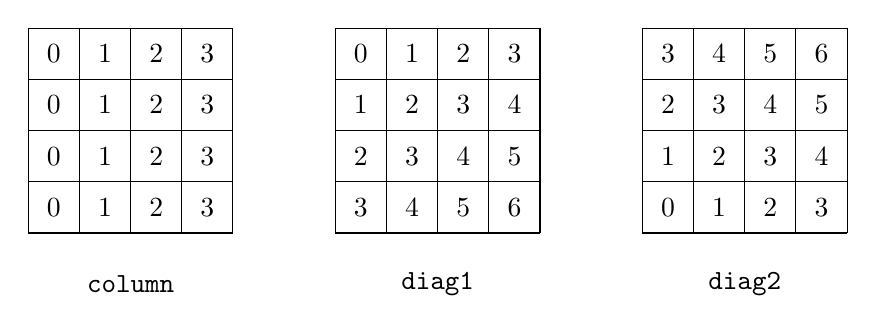
\begin{tikzpicture}[scale=.65]
  \begin{scope}
    \draw (0-6, 0) grid (4-6, 4);
    \node at (-6+0.5,3.5) {$0$};
    \node at (-6+1.5,3.5) {$1$};
    \node at (-6+2.5,3.5) {$2$};
    \node at (-6+3.5,3.5) {$3$};
    \node at (-6+0.5,2.5) {$0$};
    \node at (-6+1.5,2.5) {$1$};
    \node at (-6+2.5,2.5) {$2$};
    \node at (-6+3.5,2.5) {$3$};
    \node at (-6+0.5,1.5) {$0$};
    \node at (-6+1.5,1.5) {$1$};
    \node at (-6+2.5,1.5) {$2$};
    \node at (-6+3.5,1.5) {$3$};
    \node at (-6+0.5,0.5) {$0$};
    \node at (-6+1.5,0.5) {$1$};
    \node at (-6+2.5,0.5) {$2$};
    \node at (-6+3.5,0.5) {$3$};

    \draw (0, 0) grid (4, 4);
    \node at (0.5,3.5) {$0$};
    \node at (1.5,3.5) {$1$};
    \node at (2.5,3.5) {$2$};
    \node at (3.5,3.5) {$3$};
    \node at (0.5,2.5) {$1$};
    \node at (1.5,2.5) {$2$};
    \node at (2.5,2.5) {$3$};
    \node at (3.5,2.5) {$4$};
    \node at (0.5,1.5) {$2$};
    \node at (1.5,1.5) {$3$};
    \node at (2.5,1.5) {$4$};
    \node at (3.5,1.5) {$5$};
    \node at (0.5,0.5) {$3$};
    \node at (1.5,0.5) {$4$};
    \node at (2.5,0.5) {$5$};
    \node at (3.5,0.5) {$6$};

    \draw (6, 0) grid (10, 4);
    \node at (6.5,3.5) {$3$};
    \node at (7.5,3.5) {$4$};
    \node at (8.5,3.5) {$5$};
    \node at (9.5,3.5) {$6$};
    \node at (6.5,2.5) {$2$};
    \node at (7.5,2.5) {$3$};
    \node at (8.5,2.5) {$4$};
    \node at (9.5,2.5) {$5$};
    \node at (6.5,1.5) {$1$};
    \node at (7.5,1.5) {$2$};
    \node at (8.5,1.5) {$3$};
    \node at (9.5,1.5) {$4$};
    \node at (6.5,0.5) {$0$};
    \node at (7.5,0.5) {$1$};
    \node at (8.5,0.5) {$2$};
    \node at (9.5,0.5) {$3$};

    \node at (-4,-1) {\texttt{column}};
    \node at (2,-1) {\texttt{diag1}};
    \node at (8,-1) {\texttt{diag2}};

  \end{scope}
\end{tikzpicture}
\end{center}

Let $q(n)$ denote the number of ways
to place $n$ queens on an $n \times n$ chessboard.
The above backtracking
algorithm tells us that, for example, $q(8)=92$.
When $n$ increases, the search quickly becomes slow,
because the number of solutions increases
exponentially.
For example, calculating $q(16)=14772512$
using the above algorithm already takes about a minute
on a modern computer\footnote{There is no known way to efficiently
calculate larger values of $q(n)$. The current record is
$q(27)=234907967154122528$, calculated in 2016 \cite{q27}.}.

\section{Pruning the search}

We can often optimize backtracking
by pruning the search tree.
The idea is to add ''intelligence'' to the algorithm
so that it will notice as soon as possible
if a partial solution cannot be extended
to a complete solution.
Such optimizations can have a tremendous
effect on the efficiency of the search.

Let us consider the problem
of calculating the number of paths
in an $n \times n$ grid from the upper-left corner
to the lower-right corner such that the
path visits each square exactly once.
For example, in a $7 \times 7$ grid,
there are 111712 such paths.
One of the paths is as follows:

\begin{center}
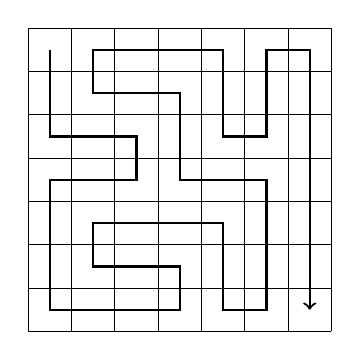
\begin{tikzpicture}[scale=.55]
  \begin{scope}
    \draw (0, 0) grid (7, 7);
    \draw[thick,->] (0.5,6.5) -- (0.5,4.5) -- (2.5,4.5) --
          (2.5,3.5) -- (0.5,3.5) -- (0.5,0.5) --
          (3.5,0.5) -- (3.5,1.5) -- (1.5,1.5) --
          (1.5,2.5) -- (4.5,2.5) -- (4.5,0.5) --
          (5.5,0.5) -- (5.5,3.5) -- (3.5,3.5) --
          (3.5,5.5) -- (1.5,5.5) -- (1.5,6.5) --
          (4.5,6.5) -- (4.5,4.5) -- (5.5,4.5) --
          (5.5,6.5) -- (6.5,6.5) -- (6.5,0.5);
  \end{scope}
\end{tikzpicture}
\end{center}

We focus on the $7 \times 7$ case,
because its level of difficulty is appropriate to our needs.
We begin with a straightforward backtracking algorithm,
and then optimize it step by step using observations
of how the search can be pruned.
After each optimization, we measure the running time
of the algorithm and the number of recursive calls,
so that we clearly see the effect of each
optimization on the efficiency of the search.

\subsubsection{Basic algorithm}

The first version of the algorithm does not contain
any optimizations. We simply use backtracking to generate
all possible paths from the upper-left corner to
the lower-right corner and count the number of such paths.

\begin{itemize}
\item
running time: 483 seconds
\item
number of recursive calls: 76 billion
\end{itemize}

\subsubsection{Optimization 1}

In any solution, we first move one step
down or right.
There are always two paths that 
are symmetric
about the diagonal of the grid
after the first step.
For example, the following paths are symmetric:

\begin{center}
\begin{tabular}{ccc}
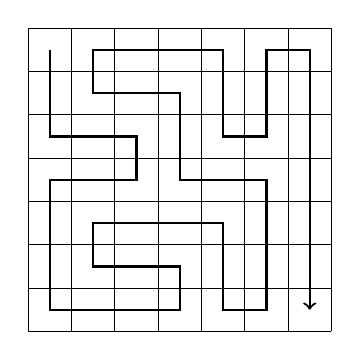
\begin{tikzpicture}[scale=.55]
  \begin{scope}
    \draw (0, 0) grid (7, 7);
    \draw[thick,->] (0.5,6.5) -- (0.5,4.5) -- (2.5,4.5) --
          (2.5,3.5) -- (0.5,3.5) -- (0.5,0.5) --
          (3.5,0.5) -- (3.5,1.5) -- (1.5,1.5) --
          (1.5,2.5) -- (4.5,2.5) -- (4.5,0.5) --
          (5.5,0.5) -- (5.5,3.5) -- (3.5,3.5) --
          (3.5,5.5) -- (1.5,5.5) -- (1.5,6.5) --
          (4.5,6.5) -- (4.5,4.5) -- (5.5,4.5) --
          (5.5,6.5) -- (6.5,6.5) -- (6.5,0.5);
  \end{scope}
\end{tikzpicture}
& \hspace{20px}
& 
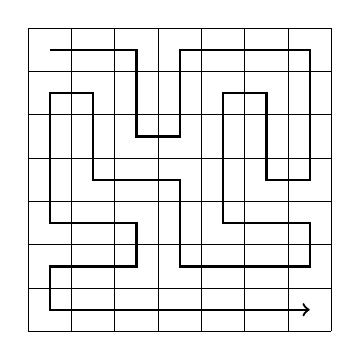
\begin{tikzpicture}[scale=.55]
  \begin{scope}[yscale=1,xscale=-1,rotate=-90]
    \draw (0, 0) grid (7, 7);
    \draw[thick,->] (0.5,6.5) -- (0.5,4.5) -- (2.5,4.5) --
          (2.5,3.5) -- (0.5,3.5) -- (0.5,0.5) --
          (3.5,0.5) -- (3.5,1.5) -- (1.5,1.5) --
          (1.5,2.5) -- (4.5,2.5) -- (4.5,0.5) --
          (5.5,0.5) -- (5.5,3.5) -- (3.5,3.5) --
          (3.5,5.5) -- (1.5,5.5) -- (1.5,6.5) --
          (4.5,6.5) -- (4.5,4.5) -- (5.5,4.5) --
          (5.5,6.5) -- (6.5,6.5) -- (6.5,0.5);
  \end{scope}
\end{tikzpicture}
\end{tabular}
\end{center}

Hence, we can decide that we always first
move one step down (or right),
and finally multiply the number of solutions by two.

\begin{itemize}
\item
running time: 244 seconds
\item
number of recursive calls: 38 billion
\end{itemize}

\subsubsection{Optimization 2}

If the path reaches the lower-right square
before it has visited all other squares of the grid,
it is clear that
it will not be possible to complete the solution.
An example of this is the following path:

\begin{center}
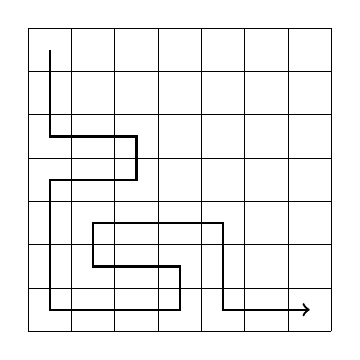
\begin{tikzpicture}[scale=.55]
  \begin{scope}
    \draw (0, 0) grid (7, 7);
    \draw[thick,->] (0.5,6.5) -- (0.5,4.5) -- (2.5,4.5) --
          (2.5,3.5) -- (0.5,3.5) -- (0.5,0.5) --
          (3.5,0.5) -- (3.5,1.5) -- (1.5,1.5) --
          (1.5,2.5) -- (4.5,2.5) -- (4.5,0.5) --
          (6.5,0.5);
  \end{scope}
\end{tikzpicture}
\end{center}
Using this observation, we can terminate the search
immediately if we reach the lower-right square too early.
\begin{itemize}
\item
running time: 119 seconds
\item
number of recursive calls: 20 billion
\end{itemize}

\subsubsection{Optimization 3}

If the path touches a wall
and can turn either left or right,
the grid splits into two parts
that contain unvisited squares.
For example, in the following situation,
the path can turn either left or right:

\begin{center}
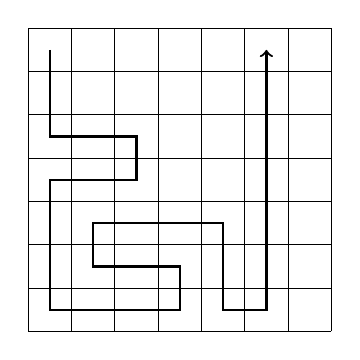
\begin{tikzpicture}[scale=.55]
  \begin{scope}
    \draw (0, 0) grid (7, 7);
    \draw[thick,->] (0.5,6.5) -- (0.5,4.5) -- (2.5,4.5) --
          (2.5,3.5) -- (0.5,3.5) -- (0.5,0.5) --
          (3.5,0.5) -- (3.5,1.5) -- (1.5,1.5) --
          (1.5,2.5) -- (4.5,2.5) -- (4.5,0.5) --
          (5.5,0.5) -- (5.5,6.5);
  \end{scope}
\end{tikzpicture}
\end{center}
In this case, we cannot visit all squares anymore,
so we can terminate the search.
This optimization is very useful:

\begin{itemize}
\item
running time: 1.8 seconds
\item
number of recursive calls: 221 million
\end{itemize}

\subsubsection{Optimization 4}

The idea of Optimization 3
can be generalized:
if the path cannot continue forward
but can turn either left or right,
the grid splits into two parts
that both contain unvisited squares.
For example, consider the following path:

\begin{center}
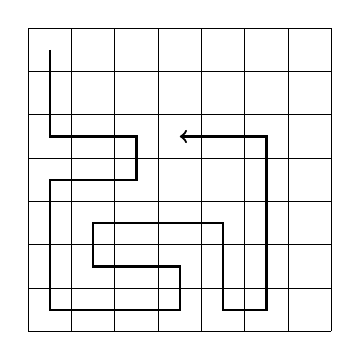
\begin{tikzpicture}[scale=.55]
  \begin{scope}
    \draw (0, 0) grid (7, 7);
    \draw[thick,->] (0.5,6.5) -- (0.5,4.5) -- (2.5,4.5) --
          (2.5,3.5) -- (0.5,3.5) -- (0.5,0.5) --
          (3.5,0.5) -- (3.5,1.5) -- (1.5,1.5) --
          (1.5,2.5) -- (4.5,2.5) -- (4.5,0.5) --
          (5.5,0.5) -- (5.5,4.5) -- (3.5,4.5);
  \end{scope}
\end{tikzpicture}
\end{center}
It is clear that we cannot visit all squares anymore,
so we can terminate the search.
After this optimization, the search is
very efficient:

\begin{itemize}
\item
running time: 0.6 seconds
\item
number of recursive calls: 69 million
\end{itemize}

~\\
Now is a good moment to stop optimizing
the algorithm and see what we have achieved.
The running time of the original algorithm
was 483 seconds,
and now after the optimizations,
the running time is only 0.6 seconds.
Thus, the algorithm became nearly 1000 times
faster after the optimizations.

This is a usual phenomenon in backtracking,
because the search tree is usually large
and even simple observations can effectively
prune the search.
Especially useful are optimizations that
occur during the first steps of the algorithm,
i.e., at the top of the search tree.

\section{Meet in the middle}

\index{meet in the middle}

\key{Meet in the middle} is a technique
where the search space is divided into
two parts of about equal size.
A separate search is performed
for both of the parts,
and finally the results of the searches are combined.

The technique can be used
if there is an efficient way to combine the
results of the searches.
In such a situation, the two searches may require less
time than one large search.
Typically, we can turn a factor of $2^n$
into a factor of $2^{n/2}$ using the meet in the
middle technique.

As an example, consider a problem where
we are given a list of $n$ numbers and
a number $x$,
and we want to find out if it is possible
to choose some numbers from the list so that
their sum is $x$.
For example, given the list $[2,4,5,9]$ and $x=15$,
we can choose the numbers $[2,4,9]$ to get $2+4+9=15$.
However, if $x=10$ for the same list,
it is not possible to form the sum.

A simple algorithm to the problem is to
go through all subsets of the elements and
check if the sum of any of the subsets is $x$.
The running time of such an algorithm is $O(2^n)$,
because there are $2^n$ subsets.
However, using the meet in the middle technique,
we can achieve a more efficient $O(2^{n/2})$ time algorithm\footnote{This
idea was introduced in 1974 by E. Horowitz and S. Sahni \cite{hor74}.}.
Note that $O(2^n)$ and $O(2^{n/2})$ are different
complexities because $2^{n/2}$ equals $\sqrt{2^n}$.

The idea is to divide the list into
two lists $A$ and $B$ such that both
lists contain about half of the numbers.
The first search generates all subsets
of $A$ and stores their sums to a list $S_A$.
Correspondingly, the second search creates
a list $S_B$ from $B$.
After this, it suffices to check if it is possible
to choose one element from $S_A$ and another
element from $S_B$ such that their sum is $x$.
This is possible exactly when there is a way to
form the sum $x$ using the numbers of the original list.

For example, suppose that the list is $[2,4,5,9]$ and $x=15$.
First, we divide the list into $A=[2,4]$ and $B=[5,9]$.
After this, we create lists
$S_A=[0,2,4,6]$ and $S_B=[0,5,9,14]$.
In this case, the sum $x=15$ is possible to form,
because $S_A$ contains the sum $6$,
$S_B$ contains the sum $9$, and $6+9=15$.
This corresponds to the solution $[2,4,9]$.

We can implement the algorithm so that
its time complexity is $O(2^{n/2})$.
First, we generate \emph{sorted} lists $S_A$ and $S_B$,
which can be done in $O(2^{n/2})$ time using a merge-like technique.
After this, since the lists are sorted,
we can check in $O(2^{n/2})$ time if
the sum $x$ can be created from $S_A$ and $S_B$.
